\newcommand{\jahr}{2019}
\documentclass[a4paper]{article}

\usepackage[T1]{fontenc}
\usepackage[utf8]{inputenc}
\usepackage{graphicx}
\usepackage{xcolor}
\usepackage{fancyhdr}

\graphicspath{{../../../materials/Vorlagen/}{images/}}
\lhead{Rechenschaftsbericht \jahr}
\rhead{\includegraphics[height=1em]{de-RSE-logo-text-colour}}
\pagestyle{fancy}

\usepackage{soul}
\usepackage{longtable}

\usepackage[breaklinks=true]{hyperref}
\def\UrlBreaks{\do\/\do-\do\ }

\usepackage{graphicx}

\renewcommand{\figurename}{Abbildung}



\begin{document}
\thispagestyle{empty}

\begin{centering}
\includegraphics[height=3em]{de-RSE-logo-text-colour}\\
\vspace{1em}
\textbf{
 \Large Rechenschaftsbericht des Vorstands\\*[.5em]
 \normalsize Geschäftsjahr: \jahr}\\*[2em]
\end{centering}

\section{Mitglieder und Mitgliedsbeiträge}

Der Verein hatte zu Beginn des Geschäftsjahres 20 und zum Ende des Geschäftsjahres 45 Mitglieder. Von diesen 45 Mitgliedern bezahlten bisher 44 (Stand 11.8.2020) ihre Beiträge für das Jahr 2019.

\section{Vorstand}

Dieser Rechenschaftsbericht wird vom Vorstand des Geschäftsjahres 2019 vorgelegt, welcher sich aus folgenden Personen zusammensetzt:

\begin{itemize}
  \setlength{\itemsep}{0pt plus 1pt}
  \item Frank Löffler (Vorsitzender)
  \item Daniel Nüst (stellvertr. Vorsitzender)
  \item Bernadette Fritzsch (Schriftführerin)
  \item Stephan Druskat (stellvertretender Schriftführer)
  \item Stephan Janosch (Schatzmeister)
  \item Martin Hammitzsch (stellvertretender Schatzmeister)
\end{itemize}

Die Anschriften können dem Gründungsprotokoll entnommen werden.

\section{2018: Rückblick}

[Um die Ereignisse im Jahr 2019 besser einordnen zu können, werden hier kurz wichtige,
vorangegangene Ereignisse beschrieben. Eine genauere Übersicht ist im Rechenschaftsbericht
2018 zu finden.]

\begin{itemize}
 \item \textbf{26.11.2018}\\
  Die \textbf{Gründungsversammlung} fand am 26. November 2018 beim Exzellenzcluster Bild Wissen Gestaltung -- Interdisziplinäres Labor der Humboldt-Universität zu Berlin in der Sophienstraße 22a, 10178 Berlin, statt.
  21 Personen nahmen teil und diskutierten die im Vorfeld erstellte Satzung und Geschäftsordnung, bevor schließlich der Verein gegründet und ein erster Vorstand gewählt wurde.
 \item \textbf{November \& Dezember 2018}\\
  Der Vorstand nahm die Arbeit auf und bereitet die Anmeldung im Vereinsregister vor.
  Bis zum Jahresende lag noch keine Informationen des zuständigen Amtsgerichts Charlottenburg vor, wodurch weitere notwendige Schritte (z.B. Vereinskonto, Beantragung der Gemeinnützigkeit) und die erste ordentliche Vorstandssitzung ins Jahr 2019 gelegt werden mussten.
\end{itemize}

\section{2019: Ereignisse im Zeitverlauf}

\begin{itemize}
 \item \textbf{1.1.}\\
  Vom Schatzmeister wird eine Bar-Kasse eröffnet, in die die
  Vorstandsmitglieder ihre Mitgliedsbeiträge vorläufig einzahlen,
  solange noch kein Konto für den Verein existiert.
  Gemeinnützigkeit kann erst nach Eintragung ins Vereinsregister beantragt
  werden. Gleiches gilt für das Vereinskonto.
 \item \textbf{7.1.}\\
  Das Amtsgericht Charlottenburg fordert Änderungen der am 26.11.2018 in der
  Gründungsversammlung beschlossenen Satzung. Der
  Vorstand macht von der ebenfalls am 26.11.2018 erteilten Ermächtigung
  Gebrauch, notwendige Änderungen in der Satzung vorzunehmen.
 \item \textbf{21.1.}\\
  Von Daniel Beiter wurden verschiedene Vorschläge für ein Vereinslogo erarbeitet, aus denen der Vorstand eine Vorauswahl trifft.
  Die drei ausgewählten Versionen werden der Community zur
  Abstimmung gestellt.
 \item \textbf{Januar}\\
  Erste lokale RSE-Gruppen in Münster und München wurden initiiert. In Münster haben sich auf Initiative von Daniel Nüst 15 Personen getroffen und es sollen weitere
  Treffen folgen, wobei der CIO der Universität das Vorhaben unterstützt.
  In München organisierten Heidi Seibold, Bernd Bischl und Tobias Webereinen runden Tisch am Leibniz-Rechenzentrum mit 35 Teilnehmern. Auch hier werden weitere Treffen folgen.
 \item \textbf{1.2.}\\
  In der Umfrage in der Community votierte eine Mehrheit
  für die Version~1 (reines Text-"`de"', links oben) der Entwürfe für ein Vereinslogo.
  Der Vorstand folgte dem Votum und nahm einstimmig diese Version an:\\
  \includegraphics[height=3em]{de-RSE-logo-text-colour}
 \item \textbf{11.3.}\\
  Der Registereintrag des Vereins ist zwar endlich angenommen, kleinere Übertragungsfehler
  müssen aber noch korrigiert werden.
  Nach Prüfung der Konditionen verschiedener Banken wird die Berliner
  Volksbank für das Vereinskonto ausgewählt. Die Formalien der Kontoeröffnung werden
  einen Zeitraum von mehreren Wochen brauchen.
  Mitglieder sollen in diesem Jahr ihren Beitrag überweisen, ab 2020 soll
  der Beitrag dann per Lastschrift eingezogen werden.
  Rocket Chat soll als neuer Kommunikationskanal Slack ablösen, wo der in
  der kostenlosen Version bereitgestellte Workspace bald voll ist. GWDG
  bietet Rocket Chat an. Der Vorstand migriert daher auf
  \href{https://chat.gwdg.de/group/derse_vorstand}{https://chat.gwdg.de/group/derse\_vorstand}.
 \item \textbf{17.5.}\\
  Das Bankkonto ist eröffnet und nutzbar.
  Für die deRSE19 Konferenz wird es einen Aufsteller/Roll-up für die Gesellschaft geben.
  Gemeinnützigkeitsantrag steht noch aus, kann aber mit vorhandenem Konto nun gestellt werden.
  Letzte Vorbereitungen für die Jahreshauptversammlung werden getroffen.
 \item \textbf{13.\&14.5.}\\
  Frank Löffler, Martin Hammitzsch, Ina Schieferdecker und Stephan Janosch stellen die von de-RSE e.V. mitgetragene Initiative\\\href{RSE4NFDI}{https://www.rse4nfdi.de/} mit einem Vortrag und einem Poster auf der NFDI Konferenz in Bonn vor. Sie sorgen dafür, dass Forschungssoftware als Teil der NFDI am zweiten Tag in einer gesonderten Session thematisiert wird.\\*[1em]
  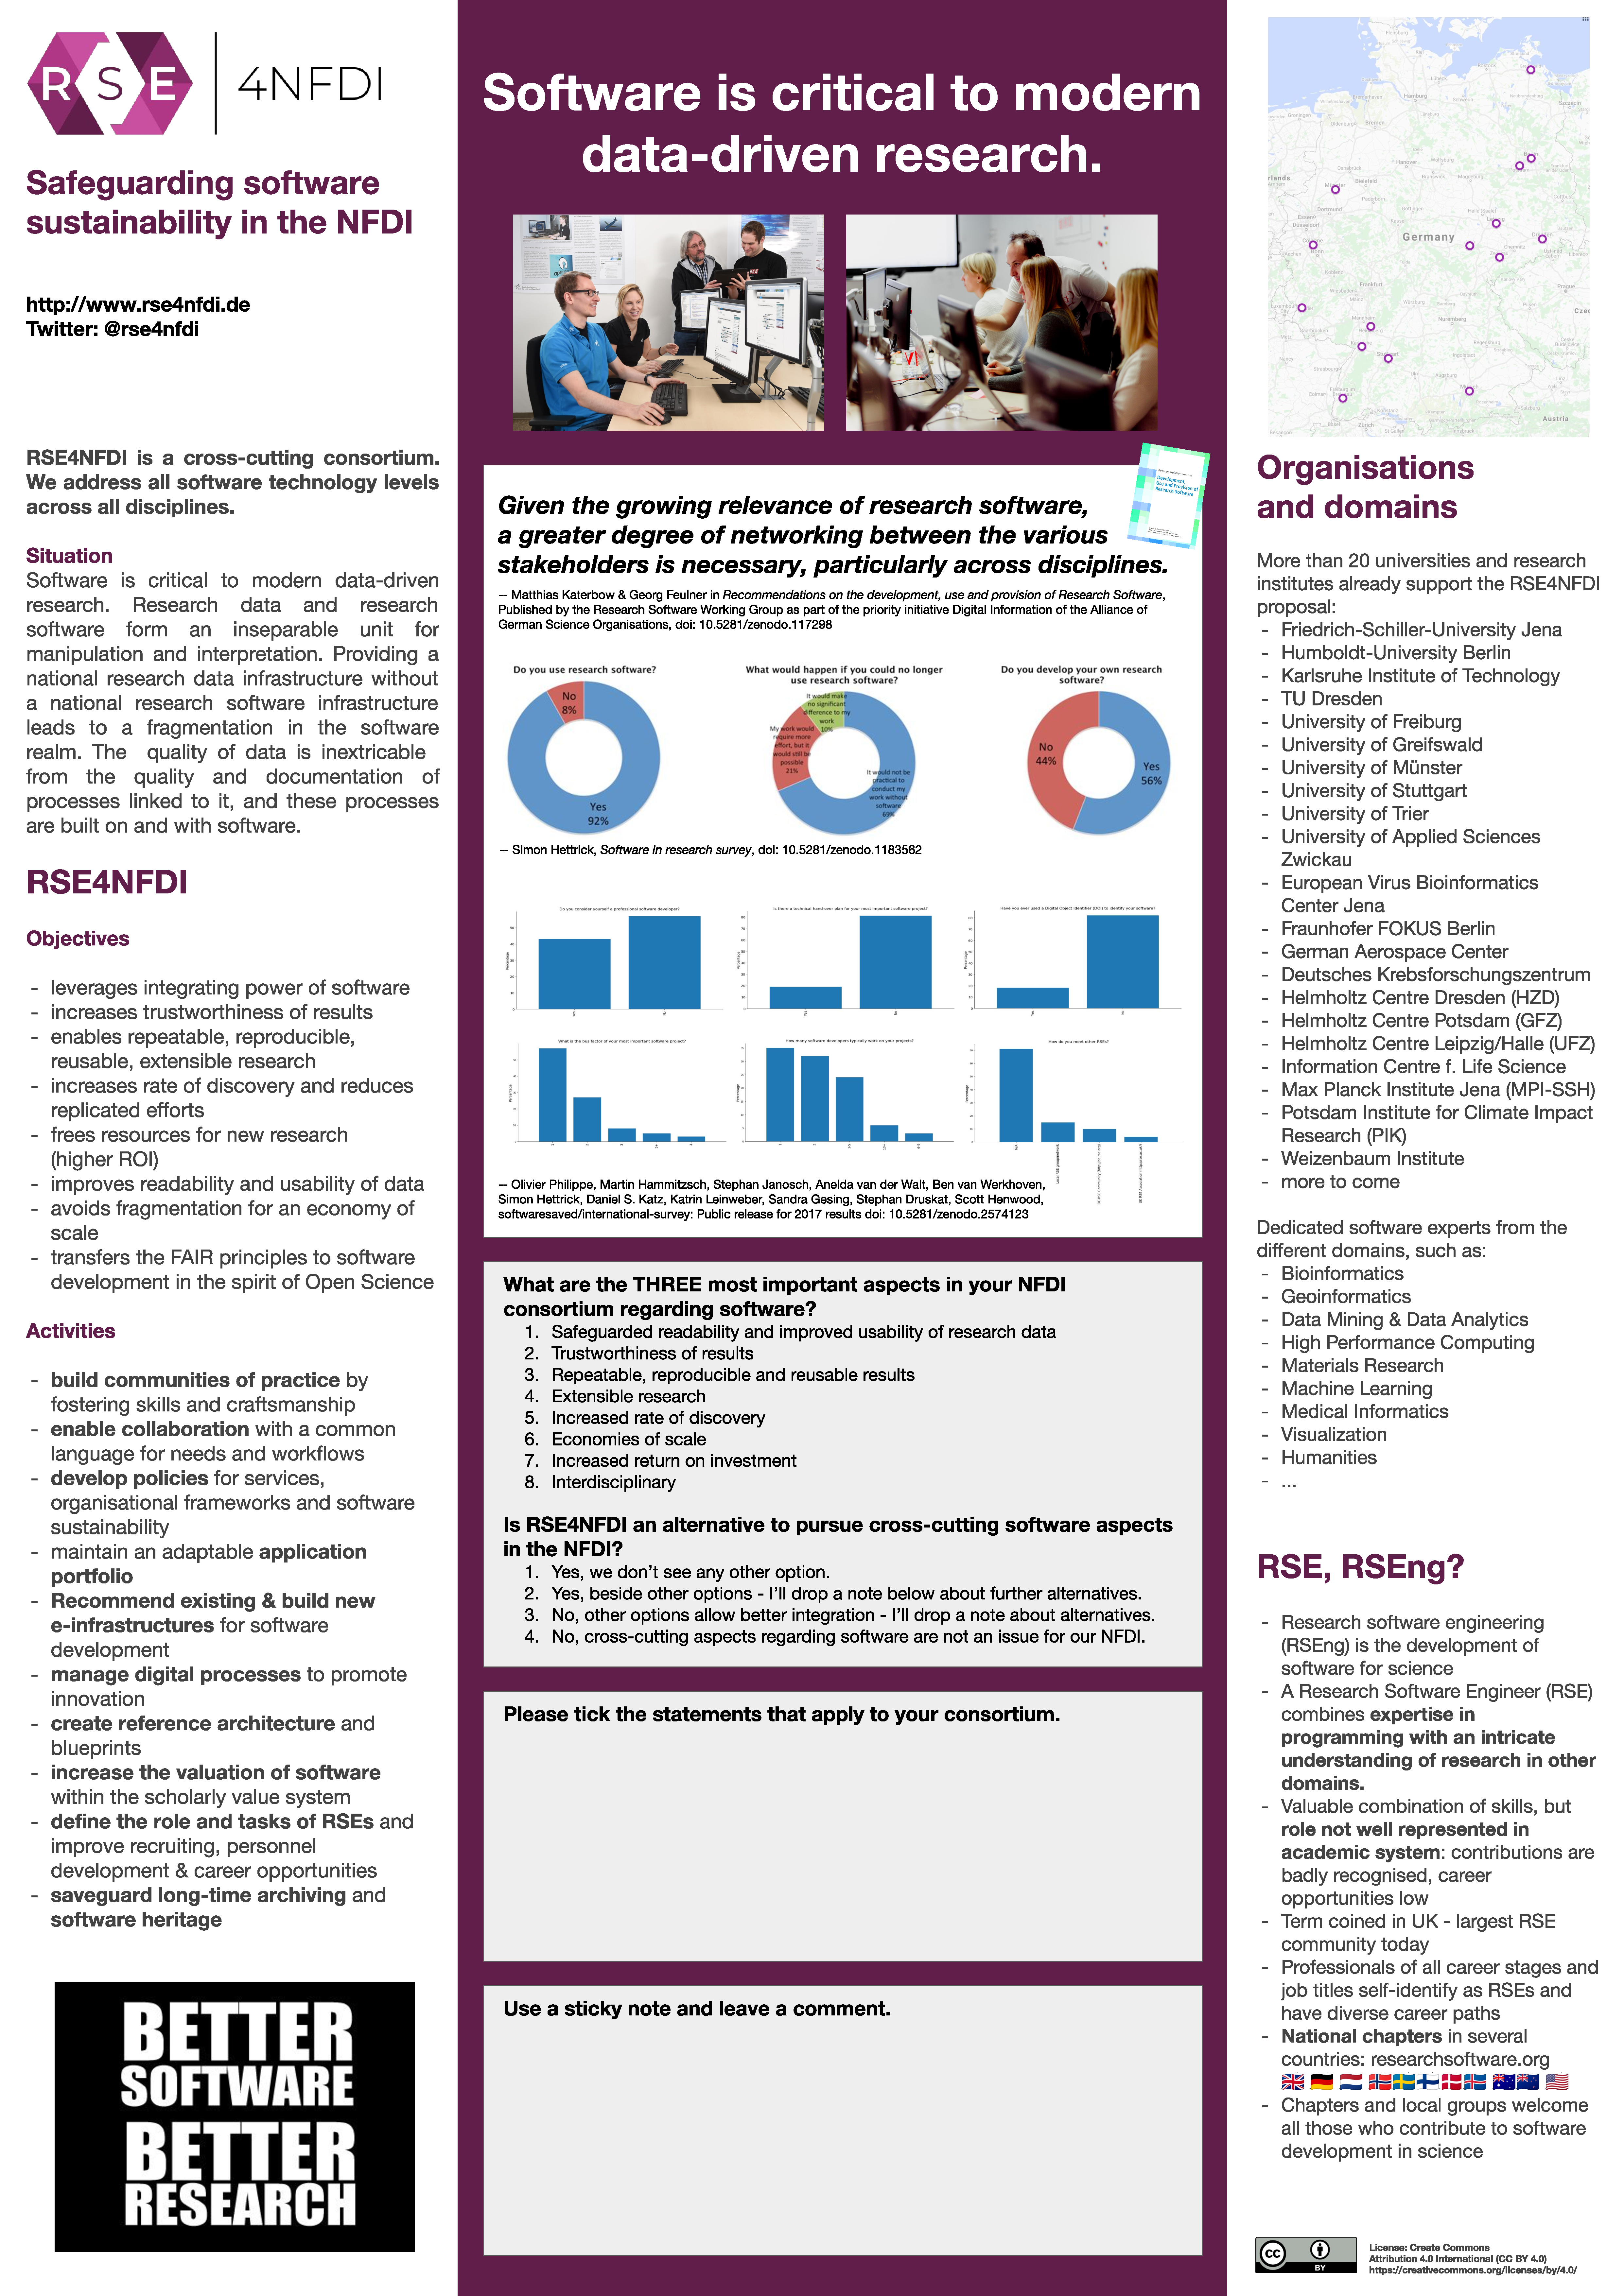
\includegraphics[width=\textwidth]{RSE4NFDI_Poster}\\
 \item \textbf{4.-6.6.}\\
 Die erste Konferenz für Forschungssoftwareentwickler/-innen in Deutschland, \textbf{deRSE19}, wird organisiert und durch unzählige Freiwillige der de-RSE-Gemeinschaft unterstützt. Die durch räumliche Gegebenheiten auf 200 begrenzte Teilnehmeranzahl wird innerhalb von 2 Wochen nach Registrierungsstart erreicht und eine Warteliste wird nötig. In Keynotes, Sessions, Workshops, BoFs, auf Postern und in korrespondierenden Lightning Talks werden bei hohen Temperaturen diverse heiße Forschungssoftware-Themen behandelt.\\
 Wir danken der Gesellschaft für Informatik e.V., die als offizieller Hauptveranstalter auftritt, und den folgenden Sponsoren: Microsoft Deutschland GmbH, Amazon Web Services, GitLab, dem R Consortium und dem Python Software Verband e.V.\\*[1em]
  \hspace*{.11\textwidth}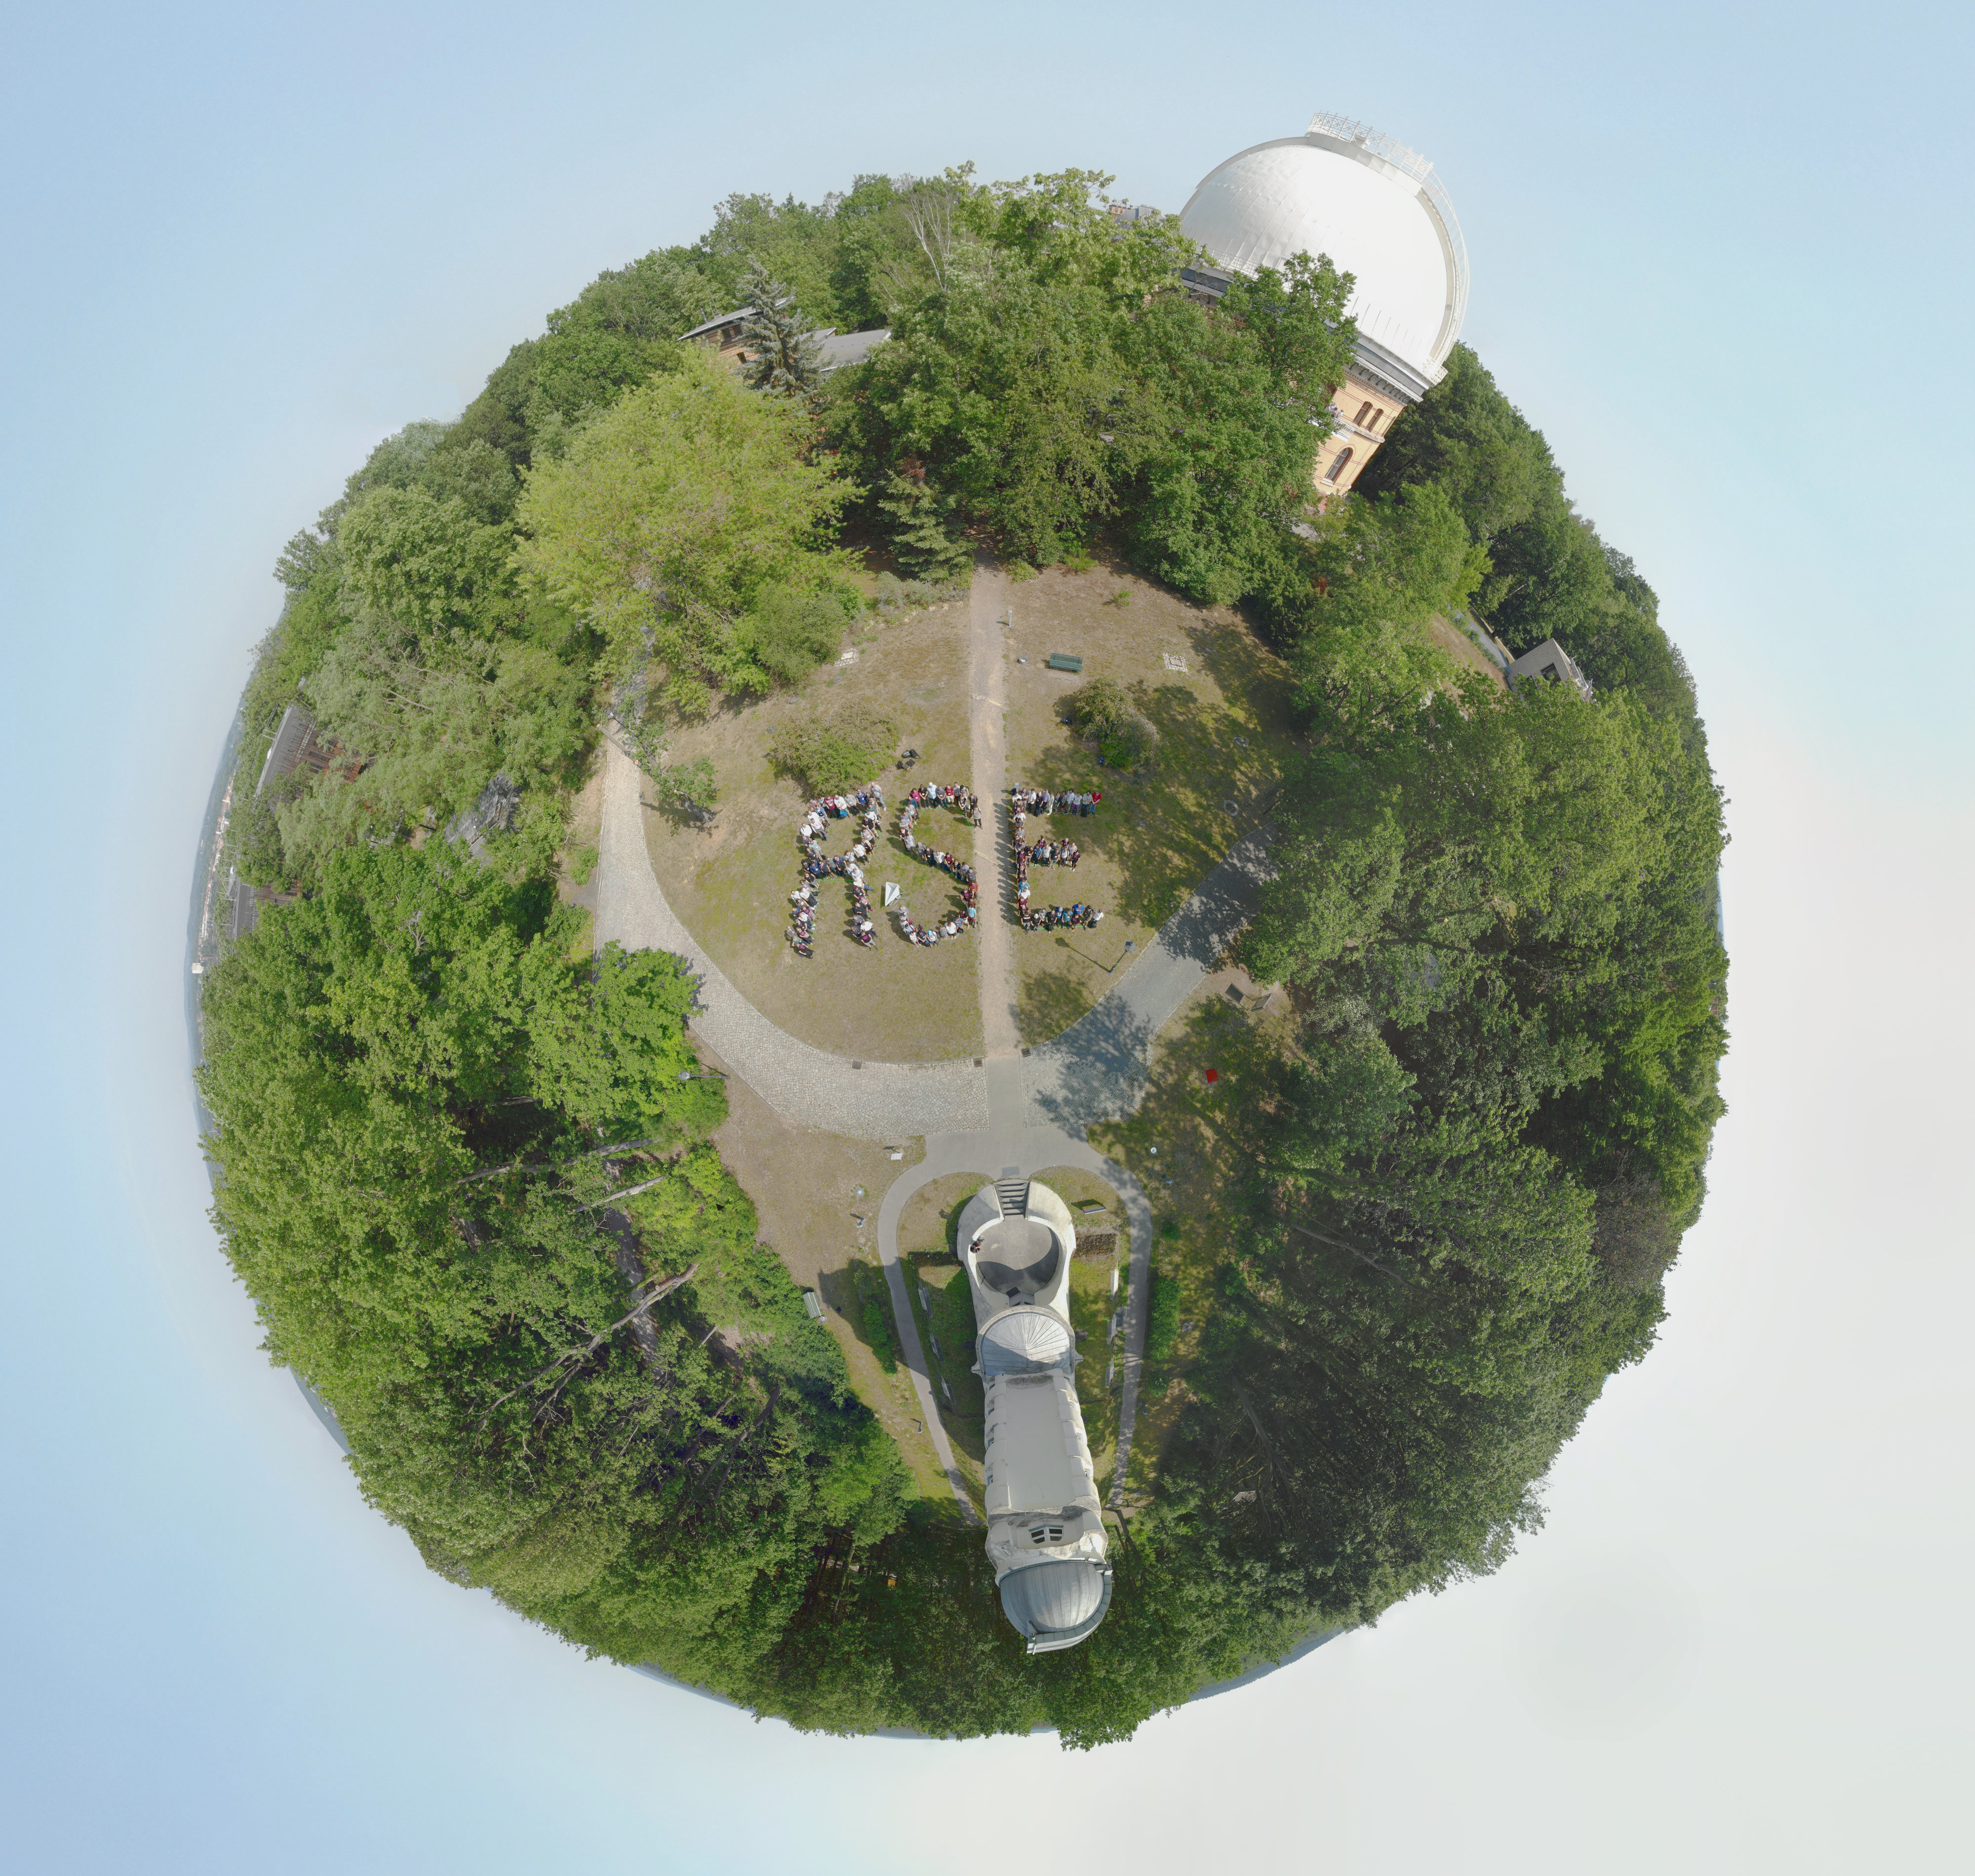
\includegraphics[width=.71\textwidth]{deRSE19_littlePlanet.jpg}\\
  \hspace*{.11\textwidth}\includegraphics[width=.71\textwidth]{deRSE19_groupPhoto1.jpg}
 \item \textbf{21.8.}\\
 Nach einer Sommerpause und Erholungspause nach der Konferenz arbeitet der Vorstand weiter an der Gemeinnützigkeit, u.a. mit Steuerberatern und Erfahrungsberichten aus anderen Vereinen. Ein Verfahren zur Veröffentlichung von Positionsverfahren wird erstellt und der Gemeinschaft zur Abstimmung vorgeschlagen.
 \item \textbf{4.9.}\\
 Der offene \href{Communityprozess zur Findung offizieller Positionen von de-RSE e.V.}{https://de-rse.org/de/positions.html} wird veröffentlicht.
 Der Prozess beinhaltet offene Calls for Contributions, kollaborative Entwicklung, öffentliche Gutachtenprozesse und darauf basierende Entscheidungen.
 \item \textbf{9.9.}\\
 Eine Kommunikationsplattform für de-RSE women wurde eingerichtet.
 Es wird an einem Antrag zu einem DFG-Rundgespräch gearbeitet: "`Nachhaltigkeit von Forschungssoftware"'.
 Mit beteiligt sind Stephan Druskat und Frank Löffler.
 Stephan Druskat präsentiert de-RSE in der RSE Worldwide Session auf der RSE Conference 2019 in Birmingham, UK. 
 Weitere de-RSE-Teilnehmer sind Carina Haupt und Tobias Schlauch.
 \item \textbf{2.10.}\\
 Der Antrag auf Gemeinnützigkeit ist zum Versandt bereit. Die Berlin-Deklaration im Zusammenhang mit der NFDI wird heftig diskutiert. Frank Löffler berichtet vom Querschnittskonsortientreffen am 1.10.2019 in Leipzig. Der de-RSE e.V. verfasst nach Anfrage einen Letter of Support für das NFDI4Chem NFDI-Konsortium. Die Planung rund um die deRSE20-Konferenz nimmt immer konkretere Formen an: Angebote werden eingeholt, notwendige Kontakte geknüpft und Call for Chairs vorbereitet.

 \item \textbf{30.10.}\\
 Mit diesem Datum hat das Finanzamt für Körperschaften I in Berlin festgestellt, dass die Satzung die Voraussetzungen für die Anerkennung der Gemeinnützigkeit erfüllt. Wir sind gemeinnützig!

 \item \textbf{4.11.}\\
 Das erste von vielen noch folgenden Treffen zur Organisation der deRSE20-Konferenz wird abgehalten.

 \item \textbf{6.11.}\\
 Ein erstes Treffen zur Gründung eines regionalen Chapters in Berlin/ Brandenburg findet statt.

 \item \textbf{7.-8.11.}\\
 Das DFG-Rundgespräch "`Nachhaltigkeit von Forschungssoftware"' findet im Robert-Koch-Institut Berlin statt.
 Ergebnis ist eine Grobfassung eines Papiers zum gleichen Thema, welches später als \href{https://arxiv.org/pdf/2005.01469.pdf}{de-RSE Position Paper 001} veröffentlicht wurde.

 \item \textbf{25.11.}\\
 Ein face-to-face Treffen des Vorstandes wird für den 8.1.2020 in Berlin organisiert. Weiterhin wird eine Bestandsaufnahme der inzwischen sehr angewachsene (digitale) Infrastruktur des Vereins durchgeführt. Dazu gehören u.a. Domainnamen, Webseiten, git-Repositories mit dazugehörigen Konten, eine sichere Dateiablage für Vereinsinterna, ein Kalender, diverse Kommunikationskanäle, eine virtuelle Maschine für die deRSE19-Konferenz, sowie JVerein für die Vereinsverwaltung.

 \item \textbf{4.12.}\\
 Frank Löffler nimmt für deRSE am NFDI-Querschnittstreffen in Berlin teil und berichtet später dem Vorstand. Allgemein größtes Problem ist die anhaltende Ungewissheit und Informationsarmut, was Querschnittsthemen innerhalb der NFDI angeht. Es wird beschlossen, die "`Berlin-Deklaration"' in einem weiteren Dokument aufzugreifen und später zu veröffentlichen. Diese beiden Dokumente werden später als "`Berlin-Leipzig-Deklaration"' benannt werden und neben anderen Querschnittsthemen auch Fragen rund um Forschungssoftware und RSEs zu einem der zentralen Punkte der nächsten NFDI-Konferenz machen.

 \item \textbf{18.12.}\\
 Vor allem für die offizielle Organisatorenrolle realer Treffen, besonders aber für die geplante deRSE20 Konferenz werden Angebote für eine Vereinshaftpflichtversicherung eingeholt und besprochen. Technische Möglichkeiten für die einfache Unterbringung von lokalen Chapterwebseiten werden diskutiert und später auch implementiert. Möglichkeiten zu de-RSE-Swag werden diskutiert. Hier stellt uns die Gemeinnützigkeit jedoch enge Grenzen und "`Workarounds"' werden diskutiert. Das nächste Vorstandstreffen Angesicht-zu-Angesicht am 8.1.2020 wird final organisiert.

\end{itemize}
\section{Weitere Ereignisse}

\begin{itemize}
 \item \textbf{Blog}
 \begin{itemize}
  \item 29.1.: \href{https://www.de-rse.org/blog/2019/01/29/umfrageverteilung-2018-in-deutschland.html}{Umfrageverteilung 2018 in Deutschland}
  \item 26.2.: \href{https://www.de-rse.org/blog/2019/02/26/new-rse-groups-meet-in-munich-and-muenster.html}{Neue RSE-Gruppen in München und Münster}
  \item 10.7.: \href{https://de-rse.org/blog/2019/07/10/derse19-ws-policies-1.html}{deRSE19: Rückblick auf den Workshop ``Entwicklung von Policies und Richtlinien für Forschungssoftware''}
  \item 26.7.: \href{https://de-rse.org/blog/2019/07/26/derse19-ws-policies-2.html}{Publikation und Zitation von Forschungssoftware - Teil 2 des deRSE19-Workshop-Rückblicks ``Entwicklung von Policies und Richtlinien für Forschungssoftware''}
  \item 22.10.: \href{https://de-rse.org/blog/2019/10/22/frauen-in-derse.html}{Frauen in de-RSE}
  \item 1.11.: \href{https://de-rse.org/blog/2019/11/01/derse20-call-for-committee-members.html}{deRSE20 Call for Committee Members}
  \item 20.12.: \href{https://de-rse.org/blog/2019/12/20/derse20-terminankuendigung.html}{Terminankündigung: deRSE20 - 2. Internationale Konferenz für research software engineers in Deutschland, 25.-27. August 2020}
 \end{itemize}
 \item \textbf{Vorstandssitzungen}\\
  Vorstandssitzungen fanden an den folgenden 15 Tagen statt: 7.1., 21.1., 1.2., 19.2., 11.3., 28.3., 17.5., 28.5, 21.8., 9.9, 2.10., 23.10., 6.11., 25.11. und 18.12. Alle Sitzungen waren beschlussfähig. Protokolle sind größtenteils öffentlich unter \href{https://github.com/DE-RSE/protokolle/}{https://github.com/DE-RSE/protokolle/} einsehbar (laut Beschluss vom 7.1.2019).
% \item \textbf{wann}\\
%  Vorstellungen von de-RSE auf Veranstaltungen
\end{itemize}

% Mindestinhalt laut https://www.vereinswelt.de/rechenschaftsbericht
%Mitgliederentwicklung: Zu- und Abgang von Mitgliedern, Erläuterungen zu auffälligen Entwicklungen, Ausschlussverfahren
%Durchgeführte Vereinsveranstaltungen
%Teilnahme an Wettbewerben und Ergebnisse
%Beziehungen zum Dachverband und zu anderen Vereinen
%Stand laufender Projekte
%Struktur des Vereins
%Aktivitäten der Organe und Ausschüsse
%Sonstige Ereignisse, die für den Verein wichtig waren
%Finanzbericht
% Empfohlen
%Beziehungen zu Sponsoren und Spendern
%Aktivitäten zur Gewinnung weiterer Sponsoren und Spender
%Ausgang von für den Verein bedeutsamen Gerichtsverfahren
%Hauptamtliche Mitarbeiter, Veränderungen im Personalbestand
%Geplante Projekte und Aktivitäten


\end{document}
